% глава 4

\chapter{Разработка алгоритма управления процессами останова и пуска конвейера} \label{chapt4}
В~данной главе рассматривается разработка и исследование работы алгоритмов управления процессами останова и пуска конвейера, которые включают в себя стабилизацию тягового фактора для устранения проскальзывания ленты при торможении конвейера и контроль провисания ленты в грузовой ветви конвейера после его останова.

Работа алгоритма управления остановом основана на предварительном торможении хвостового барабана по определенному закону для управляемого изменения натяжений ленты в точках набегания на приводной барабан и сбегания с приводного барабана. 

Алгоритм управления пуском представляет собой последовательность действий, осуществляющую пуск конвейера в условиях измененных при торможении значений натяжений ленты в ветвях конвейера с целью уменьшения нагрузки на привод во время пуска.\\

Общий принцип работы алгоритма управления остановом состоит в том, чтобы при инициировании останова конвейера осуществить торможение хвостового барабана таким образом, чтобы возникающие при этом динамические натяжения в ветвях конвейера изменили значение тягового фактора $ \frac{1}{e^{\mu\alpha}} $ до такой величины, при которой с момента отключения привода до момента останова приводного барабана проскальзывание ленты на нем будет отсутствовать. Отключение привода необходимо осуществлять после достижения значения тягового фактора определенной величины, то есть сигнал на останов привода должен быть сформирован через некоторое время после инициирования останова конвейера, определяемое скоростью распространения упругих волн в конвейерной ленте.\\

Алгоритм управления остановом можно разделить на следующие фазы:
\begin{itemize}
\item получение сигнала останова конвейера;
\item торможение хвостового барабана для создания динамических натяжений в ленте;
\item отключение привода после создания необходимых условий отсутствия проскальзывания ленты;
\item переходные процессы в ленте после останова привода, обусловленные ее механическими свойствами.\\
\end{itemize}

Для обеспечения корректного останова конвейера необходимо решить следующие задачи:
\begin{itemize}
\item выбрать величину тормозного момента хвостового барабана. Очевидно, что от величины тормозного момента зависит величина возникающих сил сопротивления движению ленты, а следовательно, величины возникающих при этом динамических натяжений. Диапазон допустимых значений тормозного момента должен быть ограничен с одной стороны минимальным значением, при котором обеспечивается необходимая величина тягового фактора, с другой стороны -- максимальным значением, при котором усилия в ленте не превышают допустимых технологических значений для ленты выбранного типа;
\item выбрать минимальное значение тягового фактора, при котором останов привода осуществляется без проскальзывания ленты. После создания дополнительных натяжений в ветвях конвейера и останова привода натяжения начинают резко изменяться, что приводит к изменению значения тягового фактора и возможному проскальзыванию ленты на приводном барабане. Поэтому необходимо обеспечить такие величины натяжений в ветвях конвейера, при которых значение тягового фактора будет удовлетворять условию Эйлера на протяжении всего времени останова привода;
\item минимизировать негативные переходные процессы в ленте после останова конвейера. К таким переходным процессам относится, прежде всего, возможное движение приводного барабана в обратном направлении под действием увеличенных натяжений в грузовой ветви, колебания скоростей сосредоточенных масс ленты, а также создание условий провисания ленты между роликоопорами грузовой ветви.
\end{itemize}




\if 0
\begin{figure} [h] 
  \center
  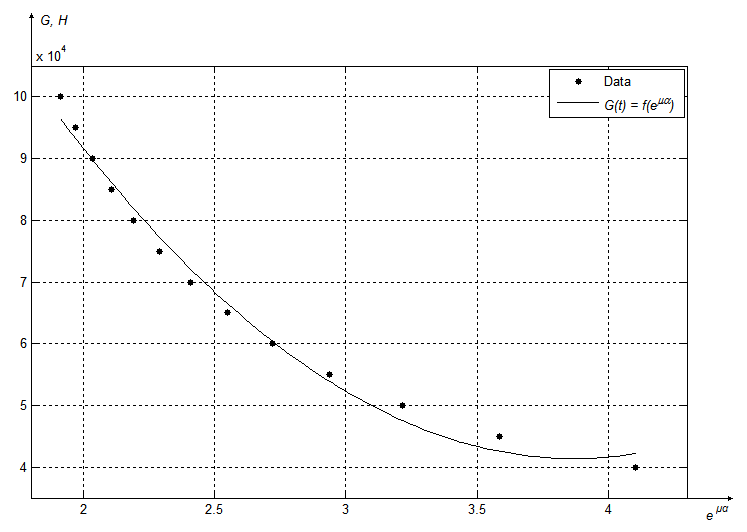
\includegraphics [scale=0.75] {4-1.png}
  \caption{Зависимость веса натяжного устройства от величины тягового фактора} 
  \label{img.4.gnu}  
\end{figure}

$$ \sigma = \sqrt{\frac{1}{n} \sum_{i=1}^n (G_{\text{ну }i} - G(t)_i)^2} $$
\fi

\section{Исследование изменения натяжений ленты конвейера при торможении хвостового барабана} \label{sect4_1}
Проведем более подробные исследования процесса торможения хвостового барабана, кратко описанные в разделе~\ref{subsect3_5_4} с целью изучения изменения натяжений ленты конвейера. Примем допущение, что груз на ленте распределен равномерно и грузопоток имеет максимальное значение, то есть конвейер полностью нагружен. 

\subsection{Общее описание процесса торможения} \label{subsect4_1_1}
В общем случае процесс торможения хвостового барабана конвейера можно описать следующим образом. При активации тормозного устройства на хвостовом барабане возникает тормозной момент, направленный противоположно направлению движения барабана. Тормозной момент создает дополнительное сопротивление движению ленты конвейера, в следствие чего появляются динамические натяжения в грузовой и порожней ветвях. При этом, в точке набегания ленты на приводной барабан в грузовой ветви натяжение увеличивается:

$$ S_{\text{гр}} = 0,5G_{\text{ну}} + W_{\text{гр}}, $$

а в точке сбегания ленты с приводного барабана в порожней ветви натяжение уменьшается:

$$ S_{\text{п}} = 0,5G_{\text{ну}} - W_{\text{п}}. $$

Здесь $ W_{\text{гр}} $ и $ W_{\text{п}} $ -- силы сопротивления движению для грузовой и порожней ветвей соответственно. Для установившегося режима работы эти силы вычисляются по формулам~\ref{eq:wgr} и~\ref{eq:wp}.

Однако, при торможении хвостового барабана конвейера возникают дополнительные динамические натяжения ленты $  \Delta S_{\text{гр}} $ и $  \Delta S_{\text{п}} $. Тогда натяжения в точках набегания ленты на приводной барабан и сбегания ленты с приводного барабана будут равны:

\begin{equation}
\label{eq:wt1}
S_{\text{гр}}' = 0,5G_{\text{ну}} + W_{\text{гр}} + \Delta S_{\text{гр}},
\end{equation}

\begin{equation}
\label{eq:wt2}
S_{\text{п}}' = 0,5G_{\text{ну}} - (W_{\text{п}} + \Delta S_{\text{п}}).
\end{equation}

Ниже показано, что возникающие при торможении хвостового барабана динамические натяжения пропорциональны силе трения между тормозной колодкой и тормозным барабаном (либо тормозным диском).\\

Рассмотрим тормозное устройство, состоящее из одного тормозного барабана и одной тормозной колодки \cite{maleksandrov1}. Общая схема такого тормозного устройства представлена на рис.~\ref{img.4.brake}.

\begin{figure} [h!] 
  \center
  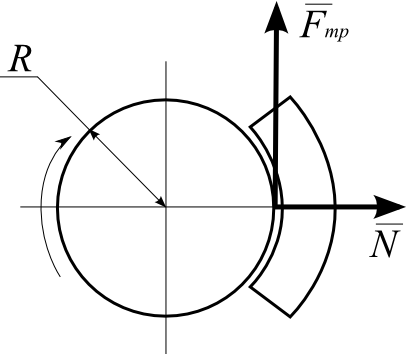
\includegraphics [scale=0.5] {4-2.png}
  \caption{Общая схема одноколодочного тормозного устройства} 
  \label{img.4.brake}  
\end{figure}

При торможении колодка прижимается к барабану с силой определенной величины, при этом возникает сила реакции опоры $ \overline{N} $, модуль которой равен модулю силы, прикладываемой к колодке, а направление -- обратное направлению силы, прикладываемой к колодке.\\

Сила трения, возникающая между колодкой и барабаном равна

$$ \overline{F}_{\text{тр}}  = \overline{N}f, $$

где $ f $ -- коэффициент трения, величина которого зависит от используемых материалов тормозного барабана и тормозной колодки~\cite{maleksandrov}. 

Тормозной момент, возникающий на хвостовом барабане конвейера, равен

$$ \overline{M}_{\text{Тхв}}  = \overline{F}_{\text{тр}} R, $$

где $ R $ -- радиус тормозного барабана. В исследуемой модели для упрощения расчетов радиус тормозного барабана принят равным радиусу хвостового барабана конвейера.\\

\subsection{Определение зависимости между динамическими натяжениями ленты и силой трения, возникающей при торможении хвостового барабана} \label{subsect4_1_2}
Чтобы показать пропорциональную зависимость между возникающими при торможении хвостового барабана динамическими натяжениями ленты и величиной силы трения, проведем несколько итераций моделирования торможения хвостового барабана конвейера при фиксированных значениях скорости движения ленты и веса натяжного устройства. Вес натяжного устройства выберем равным 80000 Н, скорость движения ленты -- 1,2 м/с. Для каждой итерации моделирования выберем определенное значение тормозного момента на хвостовом барабане.

На основе результатов моделирования были вычислены действительные значения возникающих при торможении динамических натяжений по формулам~\ref{eq:wt1} и~\ref{eq:wt2}, а также соответствующие им значения возникающей силы трения между тормозным барабаном и колодкой как отношение величины тормозного момента на хвостовом барабане к радиусу хвостового барабана. Результаты расчетов приведены в таблице~\ref{tabl:brake_data}. Помимо этого, экспериментально было установлено, что величина скорости движения ленты, изменяемая в диапазоне номинальных значений, не влияет на результаты расчета.

Последние два столбца таблицы~\ref{tabl:brake_data} содержат отношения величины динамических натяжений ленты при торможении хвостового барабана к величине сил трения между тормозным барабаном и колодкой для грузовой и порожней ветвей соответственно.

Результаты моделирования показывают, что величина возникающих при торможении хвостового барабана динамических натяжений ленты линейно зависит от силы трения, возникающей между тормозным барабаном и колодкой. Коэффициент пропорциональности не зависит от величины тормозного момента. Кроме того, модули динамических натяжений для грузовой и порожней ветвей равны между собой -- при торможении хвостового барабана конвейера натяжение в точке набегания ленты на приводной барабан в грузовой ветви увеличивается на определенную величину $\Delta S $, а натяжение в точке сбегания ленты с приводного барабана в порожней ветви уменьшается на ту же самую величину $\Delta S $.

Пусть

$$ \frac{\Delta S_{\text{гр}}}{F_{\text{тр}}} = \frac{\Delta S_{\text{п}}}{F_{\text{тр}}} = \varepsilon. $$

$ \varepsilon $ -- коэффициент пропорциональности сил сопротивления движению. Среднее значение $ \varepsilon $ на основе результатов моделирования равно 2,004. Для упрощения расчетов примем $ \varepsilon = 2. $

\begin{table}[h]
\caption{Результаты определения зависимости между силой трения, возникающей при торможении хвостового барабана и возникающими при этом динамическими натяжениями ленты.}
\label{tabl:brake_data}
\begin{center}
\begin{tabular}{|p{0.1\linewidth}|p{0.1\linewidth}|p{0.1\linewidth}|p{0.1\linewidth}|p{0.1\linewidth}|p{0.1\linewidth}|p{0.1\linewidth}|p{0.1\linewidth}|}
\hline
Тормозной момент $ M_T $, Нм & Натяжение в точке набегания $ S_{\text{гр}}' $, Н & Натяжение в точке сбегания $ S_{\text{п}}' $, Н & Величина силы трения $ F_{\text{тр}} $, Н & Динами- ческое натяжение в грузовой ветви $ \Delta S_{\text{гр}} $, Н & Динами- ческое натяжение порожней ветви $ \Delta S_{\text{п}} $, Н & $$ \frac{\Delta S_{\text{гр}}}{F_{\text{тр}}} $$ & $$ \frac{ \Delta S_{\text{п}}}{F_{\text{тр}}} $$\\
\hline
1000 & 76200 & 27463  & 2500  & 4985  & 5037  & 1,994 & 2,015 \\
1500 & 78750 & 25004  & 3750  & 7535  & 7496  & 2,009 & 1,999 \\
2000 & 81289 & 22536  & 5000  & 10074 & 9964  & 2,015 & 1,993 \\
2500 & 83787 & 20025  & 6250  & 12572 & 12475 & 2,012 & 1,996 \\
3000 & 86291 & 17523  & 7500  & 15076 & 14977 & 2,010 & 1,997 \\
3500 & 88806 & 15030  & 8750  & 17591 & 17470 & 2,010 & 1,997 \\
4000 & 91318 & 12534  & 10000 & 20103 & 19966 & 2,010 & 1,997 \\
4500 & 93813 & 10021  & 11250 & 22598 & 22479 & 2,009 & 1,998 \\
5000 & 96312 & 7512,5 & 12500 & 25097 & 24988 & 2,008 & 1,999 \\
\hline
\end{tabular}
\end{center}
\end{table}

С учетом описанных выше результатов моделирования формулы~\ref{eq:wt1} и~\ref{eq:wt2} принимают следующий вид:

\begin{equation}
\label{eq:wt3}
S_{\text{гр}}' = 0,5G_{\text{ну}} + W_{\text{гр}} + 2F_{\text{тр}},
\end{equation}

\begin{equation}
\label{eq:wt4}
S_{\text{п}}' = 0,5G_{\text{ну}} - (W_{\text{п}} + 2F_{\text{тр}}).
\end{equation}

Таким образом, используя формулу~\ref{eq:wt3} или~\ref{eq:wt4}, можно определить величину силы трения, возникающей между тормозным барабаном и колодкой при торможении хвостового барабана (а следовательно, величину тормозного момента), необходимую для того чтобы изменить натяжения ленты в ветвях конвейера до требуемых значений.

Для определения требуемой величины силы трения воспользуемся формулой~\ref{eq:wt4} для порожней ветви. Такой выбор обусловлен следующими факторами. Измерительные датчики целесообразно устанавливать на порожнюю ветвь конвейера, так как при этом минимизируется возможность повреждения датчиков транспортируемым грузом. Кроме этого, значение суммарного погонного веса $ q_{\text{п}\Sigma} $ порожней ветви, которое используется для вычисления силы сопротивления движению~(~\ref{eq:wp}), не зависит от массы транспортируемого конвейером груза и его распределения на ленте, что позволит использовать зависимость тормозного момента на хвостовом барабане от величины результирующего натяжения ленты как в случае равномерного распределения груза на ленте, так и в случае его неравномерного распределения.

Тогда величина силы трения, возникающая между тормозным барабаном и колодкой при торможении хвостового барабана, равна:

$$ F_{\text{тр}}(S_{\text{п}}') = \frac{(0,5G_{\text{ну}} - W_{\text{п}} - S_{\text{п}}')}{2}. $$

Отсюда, величина тормозного момента $ M_{\text{Тхв}} $, который требуется приложить к хвостовому барабану, чтобы величина натяжения ленты стала равной $ S_1' $, выражается следующим образом:

$$
M_{\text{Тхв}}(S_{\text{п}}') = F_{\text{тр}}(S_{\text{п}}')R_{\text{б}} = \frac{R_{\text{б}}(0,5G_{\text{ну}} - W_{\text{п}} - S_{\text{п}}')}{2}.
$$

Тогда с учетом формулы \ref{eq:wt2} выражение для тормозного момента хвостового барабана можно выразить через модуль динамического натяжения:

\begin{equation}
\label{eq:wtres}
M_{\text{Тхв}}(\Delta S) = \frac{R_{\text{б}}}{2} \Delta S.
\end{equation}

По полученной формуле можно рассчитать величину силы трения (либо тормозного момента) на хвостовом барабане по известной величине результирующего натяжения ленты для двухбарабанного ленточного конвейера с натяжным устройством, расположенным в хвостовой части. Для определения требуемой величины тормозного момента необходимо располагать следующими параметрами конвейерной установки:
\begin{itemize}
\item вес натяжного устройства $ G_{\text{ну}} $;
\item длина конвейера $ l $;
\item радиус тормозного барабана (тормозного диска) $ R_{\text{б}} $;
\item коэффициент сопротивления движению ленты $ w $;
\item погонный вес порожней ветви ленты $ q_{\text{л}} $;
\item погонный вес роликоопор в порожней ветви ленты $ q_{\text{р}} $.\\
\end{itemize}

\subsection{Моделирование процесса торможения хвостового барабана с предварительно рассчитанной величиной тормозного момента} \label{subsect4_1_3}
Для подтверждения полученных в \ref{subsect4_1_2} результатов произведем расчет требуемой величины тормозного момента, необходимой для уменьшения величины тягового фактора до значения 0,4 для конвейера, параметры которого указаны в таблице~\ref{tabl:konv_params}.

Как видно из результатов моделирования режимов работы конвейера, описанных в разделе~\ref{subsect3_5_4}, установившееся значение тягового фактора $ \frac{1}{e^{\mu\alpha}} $ при постоянной скорости движения ленты равно 0,456. При этом установившиеся значения натяжений равны $ S_{y1}(t) = 71190H, S_{y4}(t) = 32470H. $ Если к хвостовому барабану приложить тормозной момент определенной величины, будет справедливо равенство

$$ \frac{1}{e^{\mu\alpha}(t)} = \frac{S_\text{п}'(t)}{S_\text{гр}'(t)} = \frac{S_{\text{УСТ п}}(t) - \Delta S}{S_{\text{УСТ гр}}(t) + \Delta S}. $$

Подставим в это равенство числовые значения:

$$ 0,4 = \frac{32470 - \Delta S}{71190 + \Delta S}. $$

Отсюда, $ \Delta S = 2852,86 $ -- модуль модуль возникающих в ленте динамических натяжений при торможении хвостового барабана, который обеспечивает требуемую величину тягового фактора. Дополнительные натяжения именно такой величины требуется создать в ветвях конвейера посредством торможения хвостового барабана.

Рассчитаем значение тормозного момента по формуле~\ref{eq:wtres}:

$$ M_{\text{Тхв}} = \frac{0,4}{2}2852,86 = 576.572 (H). $$

Проведем моделирование торможения хвостового барабана конвейера с приложением тормозного момента вычисленной величины. На рис.~\ref{img.4.brakeE} представлен переходной процесс изменения значения тягового фактора при торможении хвостового барабана с моментом, равным 576,572 Н при движении ленты со скоростью 1,2 м/с. Торможение осуществлялось в момент времени 60 сек.

\begin{figure} [h!] 
  \center
  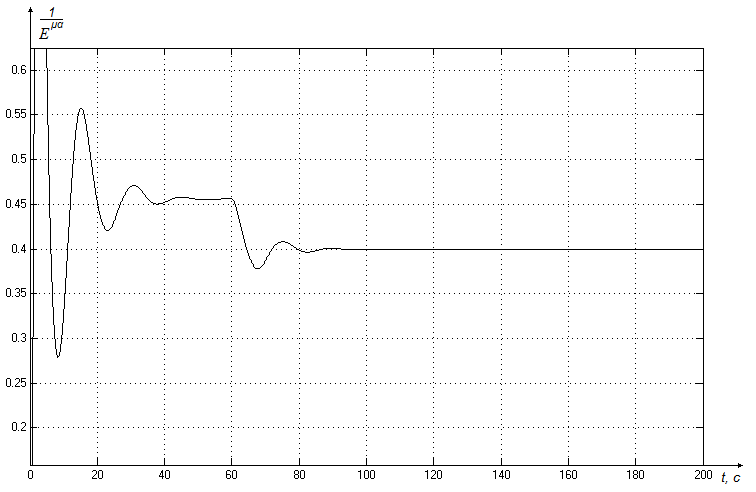
\includegraphics [scale=0.75] {4-3.png}
  \caption{Переходной процесс изменения значения тягового фактора при торможении хвостового барабана} 
  \label{img.4.brakeE}  
\end{figure}

Из графика на рис.~\ref{img.4.brakeE} видно, что после переходного процесса с колебательностью, равной 2, перерегулированием, равным 39 \% и временем регулирования, равным 30 сек, значение тягового фактора устанавливается равным предварительно заданной величине 0,4.

\subsection{Моделирование процесса останова конвейера посредством свободного выбега с предварительным торможением хвостового барабана} \label{sect4_1_4}

Если моделировать свободный выбег конвейера~(рис.~\ref{img.3.brake3}), то есть останов посредством отключения привода без использования торможения на приводном барабане, то можно видеть, что величина тягового фактора увеличивается за счет возникающих в ленте динамических усилий, связанных с остановкой движущихся частей конвейера.
В этом случае, в процессе останова привода проскальзывание ленты может иметь место, так как предварительно уменьшенная торможением хвостового барабана величина тягового фактора может превысить значение, определенное условием Эйлера.  Поэтому величину тягового фактора будем выбирать с учетом коэффициента запаса сил трения на приводном барабане $ k_T $, равного 1,1 -- 1,15 \cite{vdmitriev}.

Проведем моделирование останова конвейера посредством свободного выбега, создав предварительный тормозной момент на хвостовом барабане для обеспечения требуемой величины тягового фактора с учетом коэффициента запаса сил трения на приводном барабане $ k_T $.\\

Номинальное значение тягового фактора равно:

$$ \frac{1}{e^{\mu\alpha}} = 0,4 \cdot \frac{1}{1,15} = 0,35. $$

Тогда соответствующее ему значение тормозного момента, согласно формуле~\ref{eq:wtres}, равно $ M_{\text{Тхв}} = 1125,04 \text{Нм}. $

На рис.~\ref{img.4.brakeE1} представлен переходной процесс изменения значения тягового фактора, значение которого выбрано с учетом коэффициента запаса сил трения на приводном барабане. Торможение хвостового барабана производится с моментом, равным 1125,4 Н. 

\begin{figure} [h!] 
  \center
  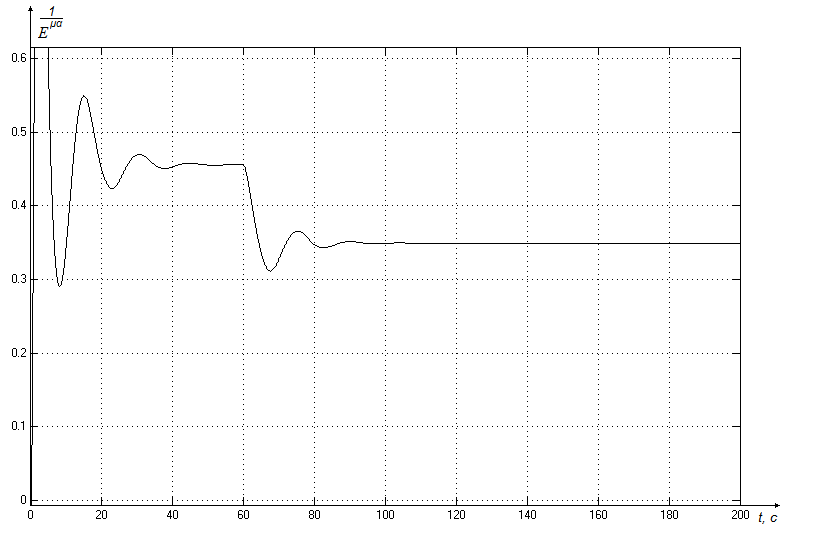
\includegraphics [scale=0.75] {4-6.png}
  \caption{Переходной процесс изменения значения тягового фактора при торможении хвостового барабана. Значение тягового фактора выбрано с учетом коэффициента запаса сил трения на приводном барабане} 
  \label{img.4.brakeE1}  
\end{figure}

Из графика на рис.~\ref{img.4.brakeE1} видно, что в момент времени 100 сек переходной процесс завершился и величина тягового фактора приняла расчетное значение, равное 0,35.

Проведем моделирование останова конвейера посредством свободного выбега с предварительным торможением хвостового барабана. Торможение хвостового барабана инициируем в момент времени 60 сек с тормозным моментом равным 1125,4 Нм, отключение привода произведем в момент времени 100 сек, когда переходной процесс изменения величины тягового фактора гарантировано завершится. Временная задержка в 40 секунд в данном случае выбрана на основе результатов моделирования стабилизации тягового фактора при торможении хвостового барабана с учетом коэффициента запаса сил трения (рис. \ref{img.4.brakeE1}).

Результаты моделирования останова конвейера посредством свободного выбега приведены на рис.~\ref{img.4.brakeE2}. Из графика видно, что при отключении привода значение тягового фактора резко возрастает, что является следствием резкого уменьшения натяжения в точке набегания ленты на приводной барабан и увеличения натяжения в точке сбегания ленты с приводного барабана. В свою очередь, это может привести к проскальзыванию ленты в определенный период останова привода, а также к провисанию ленты между роликоопорами в грузовой ветви после останова конвейера.

В данном случае проскальзывания ленты при останове конвейера не происходит. В этом можно убедиться, сравнив время останова приводного барабана и время, в течение которого значение тягового фактора после отключения привода не превышало значения~0,4~(рис.~\ref{img.4.brakeE3}). Время, в течение которого останавливался привод, $ t_o = 0,67 c $. Время, в течение которого значение тягового фактора после отключения привода не превышало значения~0,4 $ t_c = 1,14 c $. $ t_c > t_o $.\\

\begin{figure} [h!] 
  \center
  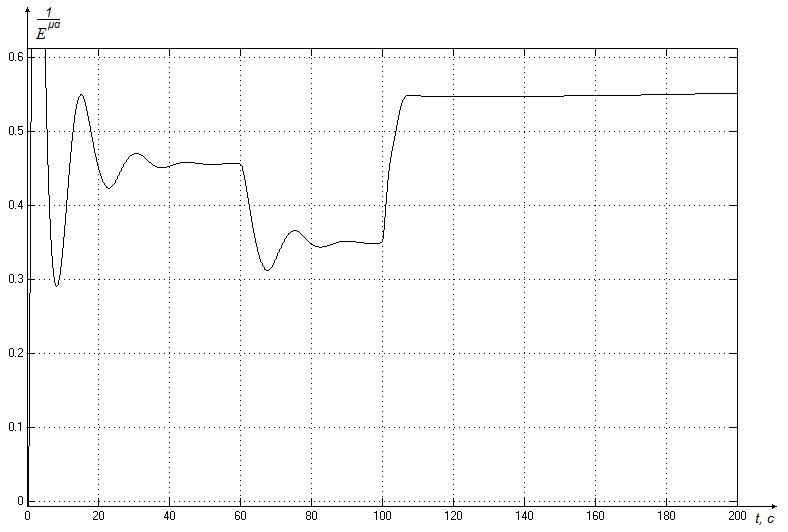
\includegraphics [scale=0.6] {4-7.png}
  \caption{Переходной процесс изменения значения тягового фактора при торможении хвостового барабана и последующем отключении привода конвейера} 
  \label{img.4.brakeE2}  
\end{figure}

\begin{figure} [h!] 
  \center
  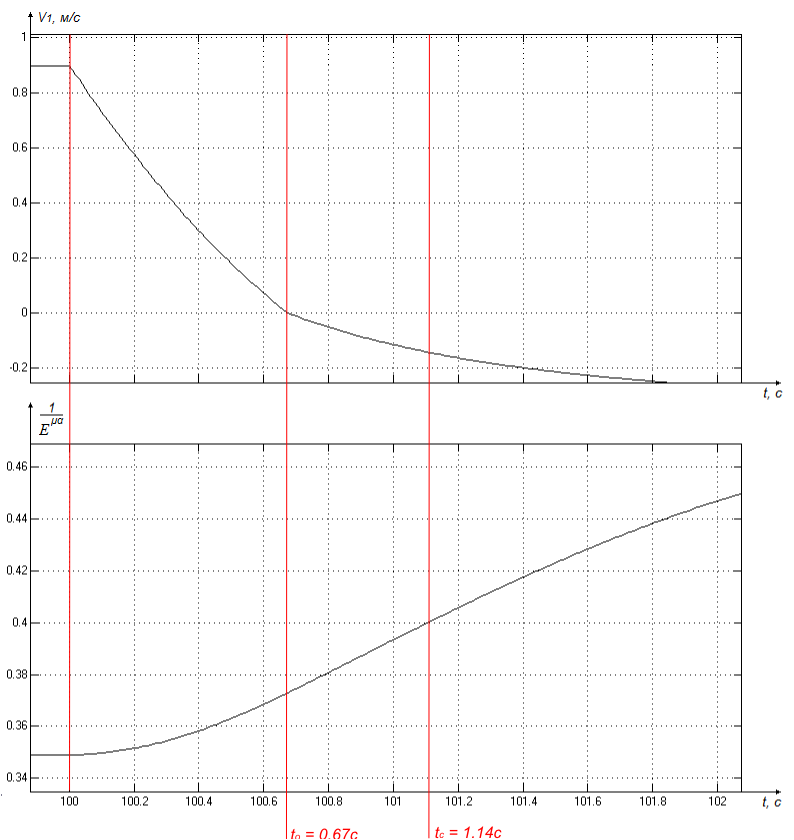
\includegraphics [scale=0.55] {4-8.png}
  \caption{Сравнение времени останова привода и времени, в течение которого значение тягового фактора после отключения привода не превышало значения~0,4} 
  \label{img.4.brakeE3}  
\end{figure}


\section{Исследование изменения натяжений ленты конвейера после останова привода} \label{sect4_2}

Изменение натяжений после останова привода происходит за счет механических свойств ленты, которая стремится принять свое нормальное состояние. Вместе с этим возможно и вращение приводного барабана в обратном направлении. На рис.~\ref{img:4.drivereverse} виден промежуток времени в течение которого скорость приводного барабана отрицательна. В этот же промежуток времени на рис.~\ref{img.4.brakeE2} наблюдается увеличение величины тягового фактора в следствие изменения натяжений. При этом, наиболее опасным является резкое уменьшение натяжения в грузовой ветви конвейера, что может привести к провисанию ленты с грузом между роликоопорами.\\

Для того чтобы не допустить уменьшения натяжения в грузовой ветви конвейера после останова привода, необходимо задействовать тормозное устройство на приводном барабане в момент его останова. При этом вращение тормозного барабана блокируется и за счет этого натяжение ленты в грузовой ветви уменьшаться не будет.

\begin{figure} [h!] 
  \center
  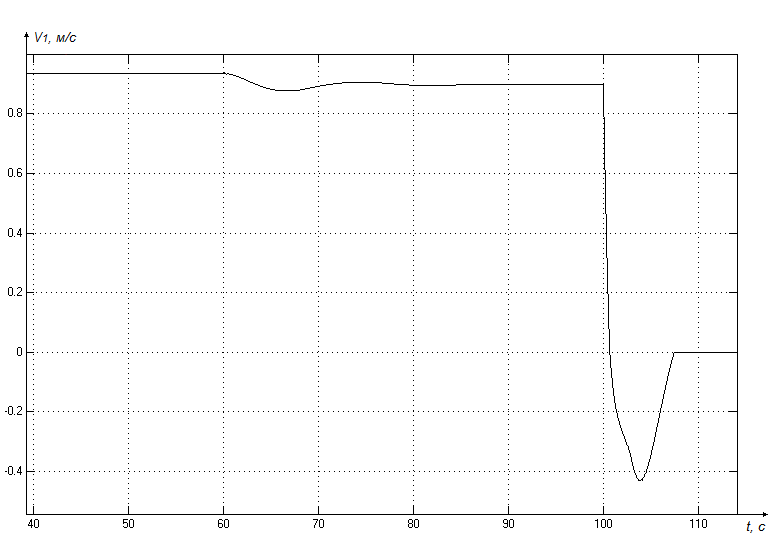
\includegraphics [scale=0.75] {4-9.png}
  \caption{Изменение скорости вращения приводного барабана при останове конвейера с предварительным торможением хвостового барабана} 
  \label{img:4.drivereverse}  
\end{figure}

%\subsection{Расчет тормозного момента для приводного барабана, обеспечивающего его блокировку после останова} \label{sect4_2_1}

Рассчитаем минимальную величину тормозного момента, необходимую для блокировки приводного барабана после его останова. Рассмотрим момент времени, когда в ветвях конвейера созданы динамические натяжения путем предварительного торможения хвостового барабана и приводной барабан остановлен~(рис.~\ref{img:4.driveM}):

\begin{figure} [h!] 
  \center
  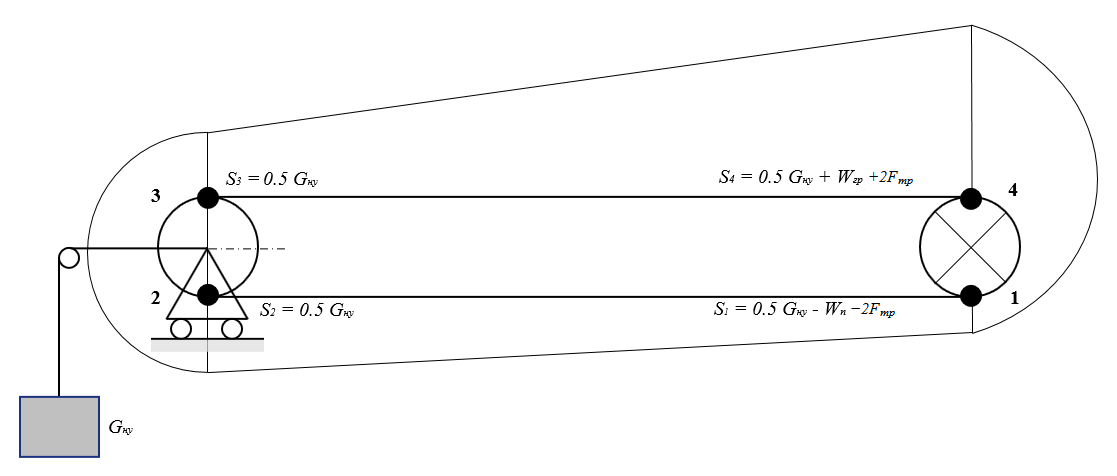
\includegraphics [scale=0.5] {4-10.png}
  \caption{Определение натяжений после останова приводного барабана} 
  \label{img:4.driveM}  
\end{figure}

Предположим, что в этой системе движение ленты осуществляется в обратном направлении, то есть грузовая ветвь ленты движется в направлении от приводного барабана к хвостовому. Рассмотрим силы, действующие на ленту в точках 1, 2, 3 и 4 (рис.~\ref{img:4.driveM}).

В точках 1 и 4 на ленту конвейера действуют силы, модули которых равны суммарным натяжениям в момент останова приводного барабана, которые можно приблизительно вычислить по формулам ~\ref{eq:wt3} и~\ref{eq:wt4}, зная приложенный к хвостовому барабану тормозной момент. Направление силы, действующей на ленту в точке 4, совпадает с направлением движения ленты. Сила, действующая на ленту в точке 1, направлена противоположно движению ленты.

В точках 2 и 3 на ленту действуют силы, модули которых равны приблизительно половине веса натяжного устройства $ S_2 = S_3 = 0,5G_\text{ну}. $ Направление силы, действующей на ленту в точке 3, совпадает с направлением движения ленты. Сила, действующая на ленту в точке 2, направлена противоположно движению ленты.

Кроме того, так как лента приводится в движение, в ней возникают силы сопротивления движению $ W_\text{гр} $ и $ W_\text{п} $ для грузовой и порожней ветвей соответственно. Направления их действия противоположны направлению движения ленты.

Тогда суммарная действующая на приводной барабан сила в момент его останова вычисляются следующим образом:

\begin{eqnarray}
F_\Sigma = S_4 - S_1 + 0,5G_{\text{ну}} - W_\text{гр} - 0,5G_{\text{ну}} - W_\text{п} =
\nonumber \\
= 0,5G_{\text{ну}} + W_{\text{гр}} + 2F_\text{тр} - 0,5G_{\text{ну}} + W_{\text{п}} + 2F_\text{тр} + 0,5G_{\text{ну}} - W_\text{гр} - 0,5G_{\text{ну}} - W_\text{п} = \nonumber \\
= 4F_\text{тр}. \nonumber
\end{eqnarray} 

% $$ M_4 = \Big(0,5G_{\text{ну}} - W_{\text{п}} - 2\frac{M_{T\text{хв}}}{R_\text{б}}\Big)R_\text{б}. $$

Так как сила трения на хвостовом барабане $ F_\text{тр} = \frac{M_{T\text{хв}}}{R_\text{б}}, $ результирующий момент сил, действующий на приводной барабан в момент его останова, равен:

\begin{equation}
\label{eq:4.mres}
% M_\Sigma = M_1 + M_4 = -R_\text{б}(W_{\text{гр}} + W_{\text{п}}) - 4M_{T\text{хв}}.
M_{T\Sigma} = 4\frac{M_{T\text{хв}}}{R_\text{б}}.
\end{equation}

Таким образом, с помощью зависимости~\ref{eq:4.mres}, зная величину приложенного к хвостовому барабану тормозного момента, получим значение суммарного момента, действующего на приводной барабан после в момент останова. Следовательно, требуемая величина тормозного момента, который необходимо приложить к приводному барабану для его блокировки, равна взятой с обратным знаком величине суммарного момента: $ M_{T\text{пр}} = -M_{T\Sigma}. $ Так как в исследуемой модели конвейера радиус хвостового барабана равен 0,4 м, то, в соответствии с зависимостью~\ref{eq:4.mres}, величина момента, требуемая для блокировки приводного барабана, должна в 10 раз превышать величину тормозного момента, приложенного к хвостовому барабану для создания предварительных натяжений в ветвях конвейера.
% = 19990 \text{Нм} $.
\if 0
%_______________________________________________________
\subsection{Моделирование блокировки приводного барабана при торможении приводного барабана} \label{sect4_2_2}

Чтобы показать корректность проведенных в разделе~\ref{sect4_2_1} расчетов, проведем несколько итераций моделирования процесса блокировки приводного барабана для различных значений тормозного момента, прикладываемого к хвостовому барабану конвейера.В качестве величин тормозного момента, прикладываемого к хвостовому барабану, возьмем несколько произвольных значений: 500 Нм, 1000 Нм, 1500 Нм, 2000 Нм. Величину тормозного момента, прикладываемого к приводному барабану для его блокировки, рассчитаем согласно разделу~\ref{sect4_2_1}.

Радиус приводного барабана $ R_\text{б} = 0,4 $ м.

Силы сопротивления движению грузовой ветки  $ W_\text{гр} = 31215 $ Н.

Силы сопротивления движению порожней ветки  $ W_\text{п} = 7500 $ Н.

Результаты расчета тормозного момента, прикладываемого к приводному барабану для его блокировки, представлены в табл.~\ref{tabl:4.resultMpr}.

\begin{table}[h!]
\caption{Результаты расчета тормозного момента, прикладываемого к приводному барабану для его блокировки.}
\label{tabl:4.resultMpr}
\begin{center}
\begin{tabular}{|p{0.3\linewidth}|p{0.3\linewidth}|}
\hline
Величина тормозного момента, прикладываемого к хвостовому барабану $ M_{T\text{хв}}, $ Hм & Величина момента, прикладываемого к приводному барабану для его блокировки после останова $ M_{T\text{пр}}, $ Hм \\
\hline
500 & 34750 \\
\hline
1000 & 39700 \\
\hline
1500 & 44660 \\
\hline
2000 & 49620 \\
\hline
\end{tabular}
\end{center}
\end{table}
%_______________________________________________________
\fi

\section{Моделирование торможения ленты конвейера с предварительным торможением хвостового барабана, остановом привода и блокировкой приводного барабана после его останова} \label{sect4_3}

Рассмотрим торможение ленты конвейера, движущейся со скоростью 1 м/с посредством предварительного торможения хвостового барабана с остановом привода и последующей блокировкой приводного барабана. Величину тормозного момента, прикладываемого к хвостовому барабану рассчитаем согласно разделу~\ref{subsect4_1_2}, величину тормозного момента, прикладываемого к приводному барабану для его блокировки рассчитаем согласно разделу~\ref{sect4_2}. Останов привода будем производить через время $ \Delta t $ после начала торможения хвостового барабана, соответствующее первому достижению величинами натяжений расчетных значений. Это время зависит от длины конвейера и скорости распространения волн деформаций в ленте. Расчет времени $ \Delta t $ не рассматривается в настоящей работе. При моделировании значение этого параметра выбирается экспериментально.\\

В соответствии с параметрами выбранной конвейерной установки, представленными в табл.~\ref{tabl:konv_params}, рассчитаем требуемые для работы алгоритма торможения параметры.

Сила сопротивления движению грузовой ветви рассчитывается по формуле~\ref{eq:wgr}:

$$  W_{\text{гр}} = q_{\text{гр} \Sigma} l w = 1040 \cdot 1000 \cdot 0,03 = 31215 H. $$

Сила сопротивления движению порожней ветви рассчитывается по формуле~\ref{eq:wp}:

$$  W_{\text{п}} = q_{\text{п} \Sigma} l w = 250 \cdot 1000 \cdot 0,03 = 7500 H. $$

Требуемое для создания натяжений необходимой величины значение тормозного момента $ M_{T\text{пр}} $, прикладываемого к хвостовому барабану, рассчитано в разделе~\ref{subsect4_1_3}. Для того, чтобы величина тягового фактора достигла значения 0,35 (с учетом коэффициента запаса сил трения), к хвостовому барабану требуется приложить тормозной момент величиной $ M_{T\text{пр}} = 1125 $ Нм.

Тогда величина тормозного момента, который требуется приложить к приводному барабану после останова для его блокировки,  $ M_{T\text{пр}} = 10M_{T\text{хв}} = 11250 $ Нм.\\

Результатами моделирования являются:
\begin{itemize}
\item график изменения величины тягового фактора~(рис.~\ref{img:4.ema});
\item графики изменения величин натяжений~(рис.~\ref{img:4.s1s4-2});
\item переходные процессы по скоростям сосредоточенных масс ленты и натяжного устройства~(рис.~\ref{img:4.speeds}).
\end{itemize}

\begin{figure} [h!] 
  \center
  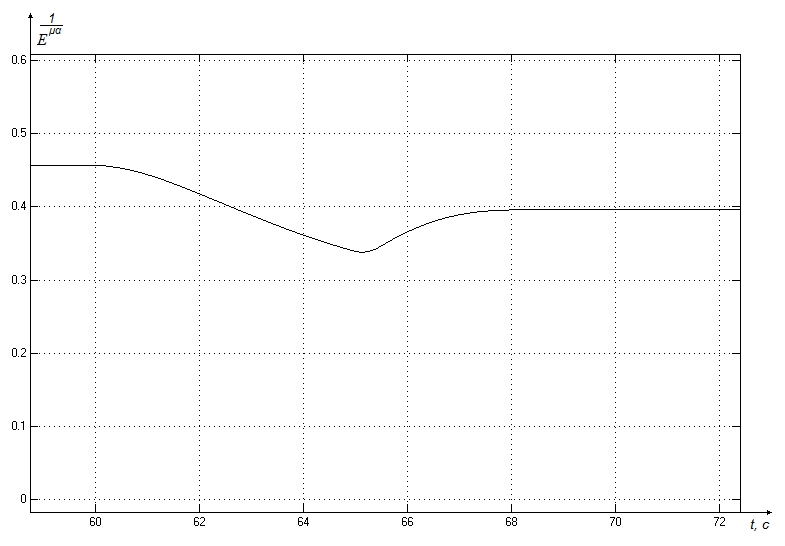
\includegraphics [scale=0.7] {4-11.png}
  \caption{График изменения величины тягового фактора при торможении ленты конвейера с предварительным торможением хвостового барабана, остановом привода и блокировкой приводного барабана после его останова} 
  \label{img:4.ema}  
\end{figure}
\clearpage

\begin{figure} [h!] 
  \center
  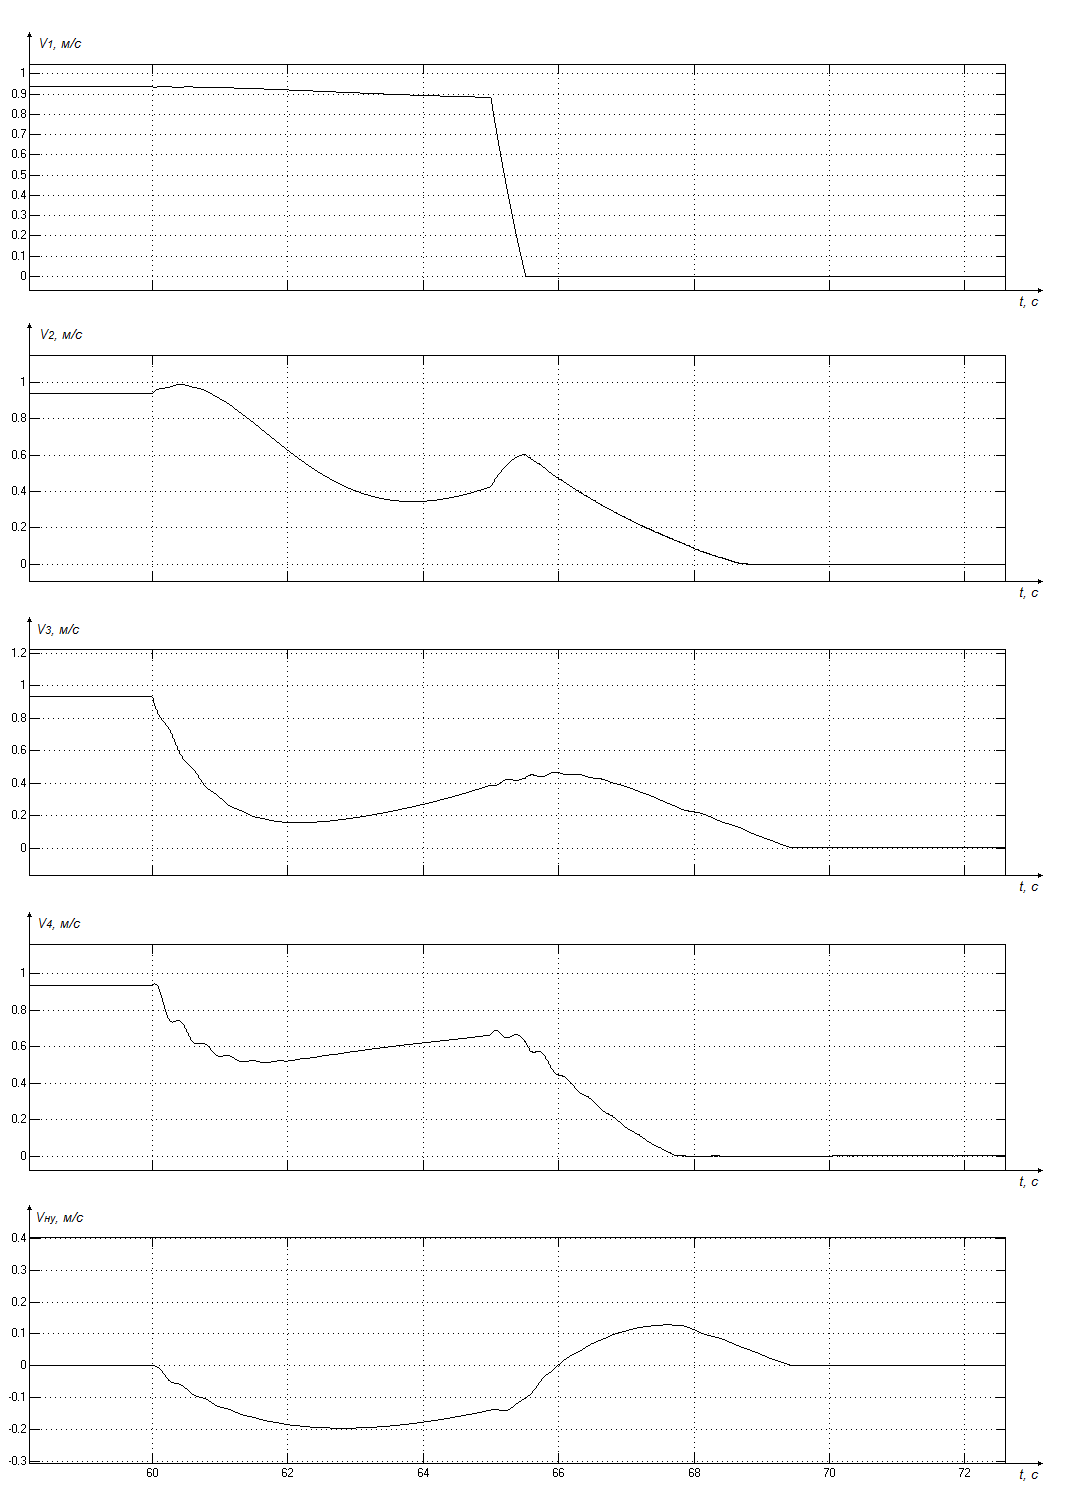
\includegraphics [scale=0.6] {4-13.png}
  \caption{Переходные процессы по скоростям сосредоточенных масс ленты и натяжного устройства при торможении ленты конвейера с предварительным торможением хвостового барабана, остановом привода и блокировкой приводного барабана после его останова} 
  \label{img:4.speeds}  
\end{figure}
\clearpage

\begin{figure} [h!] 
  \center
  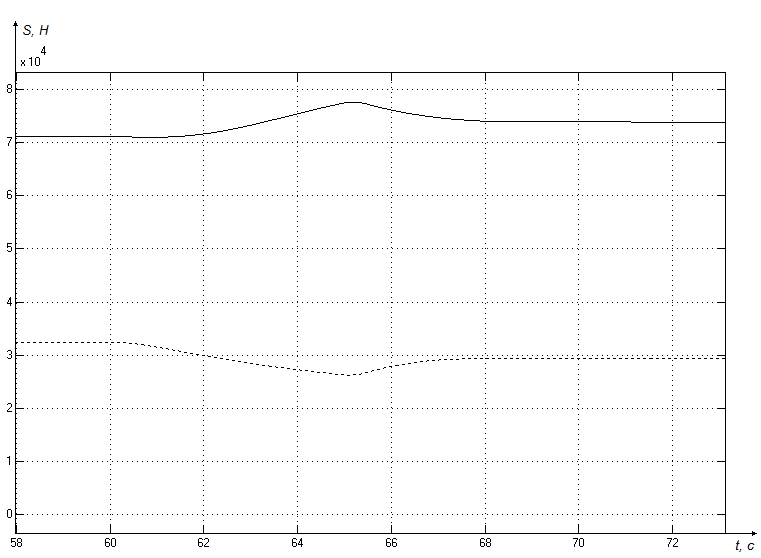
\includegraphics [scale=0.7] {4-12.png}
  \caption{Графики изменения натяжений ленты при торможении ленты конвейера с предварительным торможением хвостового барабана, остановом привода и блокировкой приводного барабана после его останова} 
  \label{img:4.s1s4-2}  
\end{figure}

\section{Исследование режима пуска конвейера после его останова с предварительным торможением хвостового барабана} \label{sect4_4}
После останова конвейера с применением разработанного алгоритма предварительного торможения в исследуемых точках ленты конвейера (точка набегания ленты на приводной барабан и точка сбегания ленты с приводного барабана) сохраняются натяжения, отличные от номинальных, определяемых весом натяжного устройства. Это имеет положительный эффект -- увеличенное, по отношению к номинальному, натяжение в грузовой ветви не позволяет ленте провисать между роликоопорами, что в свою очередь не позволяет находящемуся на ленте грузу просыпаться при последующем пуске конвейера. Условие отсутствия провисания ленты определяется по следующей формуле~\cite{vdmitriev}:

$$ S_\text{гр} \geq S_\text{доп min} = 5 \div 8(q_\text{гр} + q_\text{л})l_\text{р}, $$

где $ S_\text{гр} $ -- натяжение ленты в точке набегания ленты на приводной барабан, $ q_\text{гр} $ -- погонный вес груза, $ q_\text{л} $ -- погонный вес ленты, $ l_\text{р} $ -- расстояние между роликоопорами в грузовой ветви конвейера.\\

Если после останова конвейера отключить тормозные устройства, то это приведет к возникновению переходного процесса в ленте -- натяжение в точке набегания ленты на приводной барабан будет уменьшаться до номинального значения, определяемого весом натяжного устройства, натяжение в точке сбегания ленты с приводного барабана будет увеличиваться до номинального значения. Этот переходной процесс может сопровождаться колебаниями величин натяжений, и при этом могут возникнуть условия (возможно, кратковременные), приводящие к провисанию ленты между роликоопорами в грузовой ветви и последующему ее распрямлению, что приведет к просыпанию груза с ленты. В свою очередь, это приводит к уменьшению производительности конвейера и возможному повышению травматизма среди обслуживающего персонала.

Решить эту проблему возможно двумя способами:
\begin{itemize}
\item уменьшать тормозные моменты (отключать тормозные устройства) после останова конвейера таким образом, чтобы переходной процесс изменения натяжений в ветвях конвейера происходил без колебаний;
\item не отключать тормозные устройства, пока конвейер остановлен. При пуске конвейера одновременно с запуском привода (или с какой-либо временной задержкой) отключать тормозные устройства.
\end{itemize}

Ниже оценим пригодность и целесообразность использования каждого способа.

\subsection{Исследование отключения тормозных устройств на остановленном конвейере} \label{subsect4_4_1}
Проведем моделирование процесса изменения натяжений в ленте остановленного конвейера при одновременном отключении тормозных устройств на приводном и хвостовом барабанах. Исходным состоянием исследуемой установки будем считать состояние, когда привод остановлен, скорости сосредоточенных масс ленты равны нулю, в ветвях ленты предварительно с помощью разработанного алгоритма созданы динамические натяжения такой величины, которая требуется для стабилизации тягового фактора до значения, обеспечивающего отсутствие проскальзывания ленты при останове конвейера, тормозные устройства активированы. Конечным состоянием является состояние, при котором скорости сосредоточенных масс ленты равны нулю, тормозные устройства отключены, в ветвях ленты установились номинальные значения натяжений. Так как номинальные значения натяжений определяются весом натяжного устройства, проведем несколько итераций моделирования с различным значением веса натяжного устройства.

Результаты моделирования показали, что для любого значения веса натяжного устройства (в пределах допустимых) изменение натяжений в ветвях ленты происходит без колебаний, то есть значение натяжения в точке набегания ленты на приводной барабан никогда не становится ниже номинального, а значение натяжения в точке сбегания ленты с приводного барабана никогда не превышает номинального.

В качестве одного из результатов моделирования на рис.~\ref{img:4-4-1.s1s4} приведены графики переходных процессов по величинам натяжений для конвейера с натяжным устройством весом $ 80000 H $. На рис~\ref{img:4-4-1.speeds} приведены графики переходных процессов по скоростям сосредоточенных масс. Сигнал на останов конвейера был инициирован в момент времени $ t_1 = 60 c $, отключение тормозных устройств было инициировано в момент времени $ t_2 = 80 c $. Длительность переходного процесса (время регулирования) составляет 4 секунды для порожней ветви и 5 секунд для грузовой ветви. Перерегулирование и колебательность отсутствуют.

\begin{figure} [h!] 
  \center
  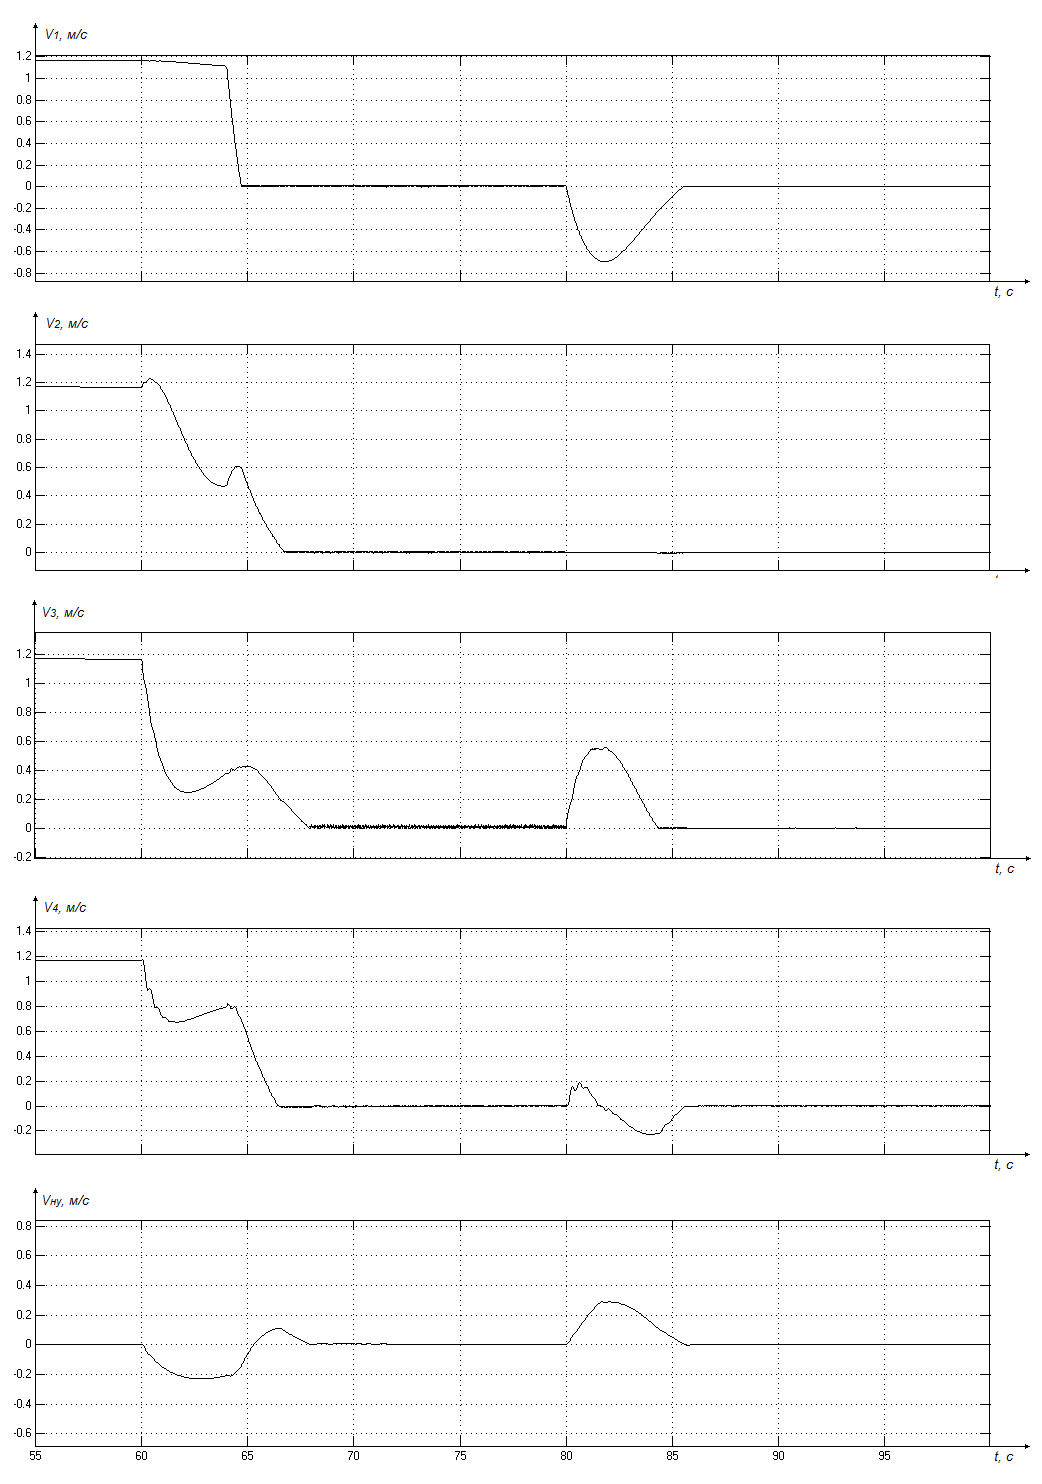
\includegraphics [scale=0.6] {4-4-2.png}
  \caption{Переходные процессы по скоростям сосредоточенных масс ленты и натяжного устройства при отключении тормозных устройств остановленного конвейера} 
  \label{img:4-4-1.speeds}  
\end{figure}
\clearpage

\begin{figure} [h!] 
  \center
  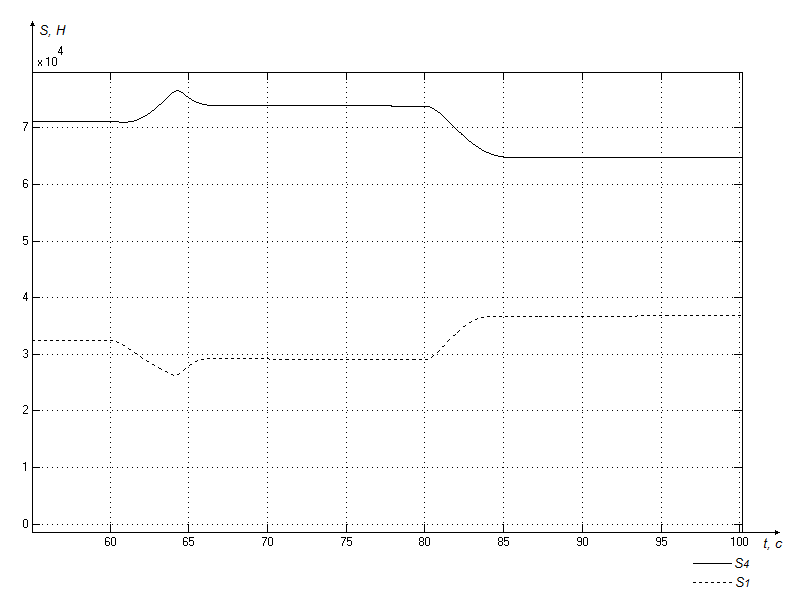
\includegraphics [scale=0.7] {4-4-1.png}
  \caption{Графики изменения натяжений ленты при  при отключении тормозных устройств остановленного конвейера} 
  \label{img:4-4-1.s1s4}  
\end{figure}

Полученные результаты моделирования говорят о том, что отключение тормозных устройств после полного останова конвейера не оказывает никакого негативного эффекта на последующий пуск конвейера и на эффективность его работы в целом. Поэтому для пуска конвейера после его остановка с помощью разработанного алгоритма предварительного торможения могут без ограничений использоваться известные алгоритмы.

\subsection{Исследование пуска конвейера с одновременным отключением тормозных устройств} \label{subsect4_4_2}
Проведем моделирование пуска остановленного конвейера при одновременном отключении тормозных устройств на приводном и хвостовом барабанах с целью исследования переходных процессов во время пуска. Исходным состоянием исследуемой установки будем считать состояние, когда привод остановлен, скорости сосредоточенных масс ленты равны нулю, в ветвях ленты предварительно с помощью разработанного алгоритма созданы динамические натяжения такой величины, которая требуется для стабилизации тягового фактора до значения, обеспечивающего отсутствие проскальзывания ленты при останове конвейера, тормозные устройства активированы. Конечным состоянием является состояние, при котором скорости сосредоточенных масс ленты равны номинальным (лента движется с номинальной скоростью), тормозные устройства отключены, в ветвях ленты установились номинальные значения натяжений.

В качестве результата моделирования рассмотрим переходной процесс скорости первой сосредоточенной массы (скорость приводного барабана), представленный на рис.~\ref{img:4-4-3.v1}. Пуск привода осуществлялся в момент времени, равный 80 сек., одновременно с этим были отключены оба тормозных устройства.

\begin{figure} [h!] 
  \center
  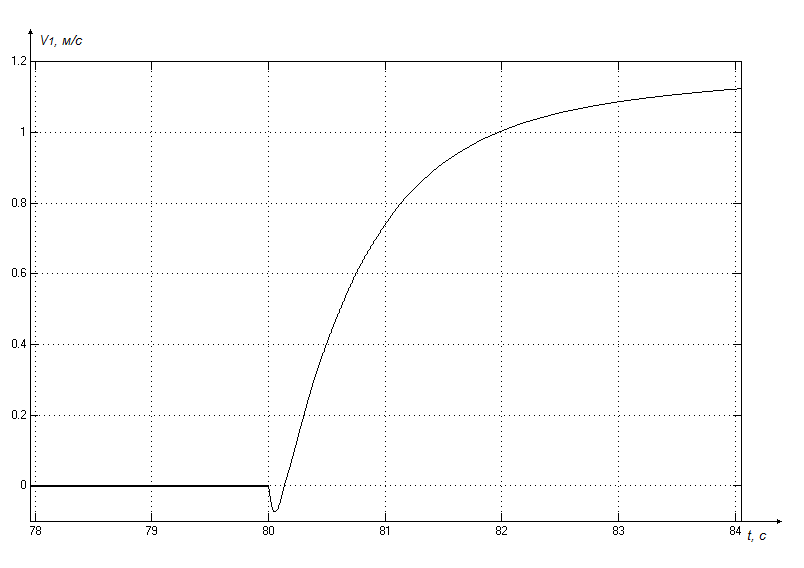
\includegraphics [scale=0.7] {4-4-3.png}
  \caption{Графики изменения натяжений ленты при  при отключении тормозных устройств остановленного конвейера} 
  \label{img:4-4-3.v1}  
\end{figure}

Из графика на рис.~\ref{img:4-4-3.v1} видно, что скорость приводного барабана в первые моменты времени отрицательна, то есть приводной барабан сначала движется в обратную сторону при работающем приводе. Это говорит о том, что первые моменты времени после старта привода момент, создаваемый натяжениями в ленте, превышает момент привода. Это практически не влияет на эффективность работы конвейера в плане процесса пуска и движения ленты, но может быть причиной повышенных нагрузок на привод, что уменьшит срок его службы.

По этой причине будем считать результаты, описанные в п.~\ref{subsect4_4_1} более приемлемыми и использовать именно их при реализации комплексной системы управления конвейером.

\section{Описание общей методики расчета параметров для работы алгоритма останова конвейера с предварительным торможением хвостового барабана} \label{sect4_5}
Учитывая описанные выше исследования, приведем общую методику расчета параметров для алгоритма останова конвейера с предварительным торможением хвостового барабана. Эта методика позволит рассчитывать параметры алгоритма для конвейеров различных модификаций на основе их характеристик. При этом предполагается, что исследуемый конвейер оборудован тормозными устройствами на приводном и хвостовом барабанах, которыми можно управлять в произвольные моменты времени.

Для работы алгоритма требуются числовые значения следующих параметров:
\begin{itemize}
\item номинальное значение тягового фактора $ \frac{1}{E^{\mu\alpha}} $, при котором гарантировано отсутствует проскальзывание ленты во время останова привода;
\item величина тормозного момента $ M_{\text{Тхв}} $, создаваемого тормозным устройством хвостового барабана, требуемая для достижения номинального значения тягового фактора $ \frac{1}{E^{\mu\alpha}} $;
\item величина тормозного момента $ M_{\text{Тпр}} $, создаваемого тормозным устройством приводного барабана, требуемая для блокировки приводного барабана после его останова;
\end{itemize}

Характеристики конвейерной установки, необходимые для расчета параметров алгоритма:
\begin{itemize}
\item длина конвейера $ L $;
\item угол обхвата лентой приводного барабана $ \alpha $;
\item коэффициент сопротивления движению ленты $ w $ (зависит от типа используемой ленты и барабанов конвейера);
\item коэффициент трения скольжения между лентой и барабаном $\mu $ (зависит от типа используемой ленты и барабанов конвейера);
% \item вес ленты грузовой ветви $ q_\text{л гр} $;
%\item вес роликоопор грузовой ветви $ q_\text{р гр} $;
\item погонный вес ленты порожней ветви $ q_\text{л} $;
\item вес роликоопор порожней ветви $ q_\text{р} $;
\item вес натяжного устройства $ G_\text{ну} $;
\item радиус тормозного барабана (диска) $ R $.
\end{itemize}

Предельное значение тягового фактора вычисляется по формуле:

$$ E_0 = \frac{1}{e^{\mu \alpha}}. $$

В реальных условиях для обеспечения отсутствия проскальзывания ленты необходим некий запас по величине тягового фактора, который учитывается с помощью коэффициента $ k_T $. В соответствии с рекомендациями~\cite{vdmitriev} его значение выбирается в диапазоне $ 0,9 \div 0,8 $. Результирующая формула определения требуемой для отсутствия проскальзывания величины тягового фактора следующая:

\begin{equation}
\label{eq:4.5.e}
E_0 = k_T \frac{1}{e^{\mu \alpha}}.
\end{equation}

Для расчета значения тормозного момента, который требуется приложить к хвостовому барабану для стабилизации тягового фактора до величины $ E_0 $, сначала рассчитывается величина динамических натяжений, которые необходимо создать в ветвях конвейера. Согласно разделу~\ref{subsect4_1_3}, справедливо следующее равенство:

$$ E_0 = \frac{S_\text{устП} - W_T}{S_\text{устГР} + W_T}, $$

где $ W_T $ -- величина динамических натяжений, $ {S_\text{устГР}} $ и $ {S_\text{устП}} $ -- значения натяжений в грузовой и порожней ветвях в установившемся режиме соответственно. Значения натяжений измеряются в реальном времени с помощью измерительных устройств (датчиков), размещенных в конвейерной установке. Тогда величина динамических натяжений, которые необходимо создать в ветвях конвейера, вычисляется по следующей формуле:

\begin{equation}
\label{eq:4.5.wt}
W_T = \frac{S_\text{устП} - E_0 S_\text{устГР}}{E_0 + 1}.
\end{equation}

Величина тормозного момента, который требуется приложить к хвостовому барабану для стабилизации тягового фактора до величины $ E_0 $, рассчитывается по формуле~\ref{eq:wtres}:

\begin{equation}
\label{eq:4.5.mtail}
M_{\text{Тхв}} = \frac{R(0,5G_{\text{ну}} - (q_{\text{л}} + q_{\text{р}})Lw - S_\text{уП} + W_T)}{2}.
\end{equation}

Величина тормозного момента, который требуется приложить к приводному барабану для его блокировки после останова привода, рассчитывается по формуле~\ref{eq:4.mres}

\begin{equation}
\label{eq:4.5.mdrive}
% M_\Sigma = M_1 + M_4 = -R_\text{б}(W_{\text{гр}} + W_{\text{п}}) - 4M_{T\text{хв}}.
M_{T \text{пр}} = 4\frac{M_{T\text{хв}}}{R}.
\end{equation}

\section{Исследования работы алгоритма предварительного управляемого торможения конвейера в зависимости от загруженности конвейера} \label{sect4_6}

Математическая модель ленточного конвейера, рассматриваемая в настоящей работе, описывает конвейер, работающий при полной нагрузке. Масса груза на ленте учитывалась при построении модели \cite{vdmitrieva1}, так как от массы груза на ленте зависит кинетическая энергия системы, а уравнения движения в модели представлены системой дифференциальных уравнений, составленных по общей схеме уравнения Лагранжа второго рода \cite{izapenin1}:
 
$$ \frac{d}{dt}\Big( \frac{\partial}{\partial \dot x_i}T \Big) - \Big( \frac{\partial}{\partial x_i}T \Big) + \frac{\partial}{\partial x_i}\textit{\text{П}} + \frac{\partial}{\partial x_i}A = 0. $$

Кинетическая энергия любого участка ленты длиной $ l $ c распределенной массой $ \frac{G}{g} $ определяется следующим образом. Пусть $ dz $ -- элементарный участок ленты на расстоянии $ z $ от начала отсчета, выделенный из участка $ x_1 x_2 $. Скорость перемещения элементарного участка $ dz $ равна $ v $, причем $ \dot x_1 < v < \dot x_2 $. В работе \cite{vdmitrieva} показано, что 

$$ \frac{\dot x_i - v}{z} = \frac{\dot x_i - \dot x_j}{l}, $$

откуда 

$$ v = \dot x_i - \frac{\dot x_i - \dot x_j}{l}z. $$

Тогда кинетическая энергия элементарного участка $ dz $ длиной $ l $ равна:

$$ dT = \frac{G_{ij}v^2}{2g}dz = \frac{G_{ij}}{2g} \Big( \dot x_i - \frac{\dot x_i - \dot x_j}{l}z \Big)^2 dz. $$

Значение кинетической энергии для распределенных масс каждого участка ленты получено интегрированием выражения для $ dT $ в пределах от 0 до $ l $:

$$ T_{ij} = \int_0^l \frac{G_{ij}}{2g} \Big( \dot x_i - \frac{\dot x_i - \dot x_j}{l}z \Big)^2 dz = \frac{G_{ij}l}{6g}(\dot x_i^2 + \dot x_i \dot x_j + \dot x_j^2), $$

где $ G_{ij} $ -- вес ленты, вращающихся частей роликоопор и груза на участке $ ij $, $ l $ -- длина участка, $ g $ -- ускорение свободного падения.
\\

При расчетах (приложение \ref{Appendix0}) величина $ \frac{G_\text{г}l}{6g} = m_\text{г} $ принята постоянной и равной 870,8 кг/м. Это значение соответствует максимальной расчетной величине грузопотока для конвейера типа 1Л-100К (420 т/час).\\

В работе \cite{alobacheva} рассмотрены основные принципы построения и исследования систем непрерывного и дискретного регулирования скорости полотна ленточного конвейера на основании вероятностных характеристик случайного шахтного грузопотока. В данной работе изложена методика определения основных параметров дискретного управления, в частности методика определения количества уровней, на которые целесообразно разделись диапазон изменения грузопотока при регулировании скорости конвейера. Воспользуемся при веденной в работе методикой для аналогичного разделения диапазона изменения грузопотока с целью исследования работы алгоритма торможения с различной загруженностью ленты.

Примем допущение, что при любом значении входящего грузопотока груз на ленте конвейера распределен равномерно. Тогда можно говорить о линейной зависимости параметра $ m_\text{г} $ от величины входящего грузопотока $ Q $. Отсутствию груза на ленте соответствует значение параметра $ m_\text{г} = 38,8 $ кг/м. По этим двум точкам составим уравнение линейной зависимости параметра $ m_\text{г} $ от величины реального грузопотока $ Q $, используя уравнение прямой следующего вида:

$$ \frac{x - x_0}{x_1 - x_0} = \frac{y - y_0}{y_1 - y_0}. $$

Полученная зависимость имеет следующий вид:

$$ m_\text{г}(Q) = 1,98Q + 38,8. $$

По полученной зависимости можно определить значение параметра $ m_\text{г} $, соответствующей средней величине грузопотока 240 т/ч: $ m_\text{г} = 514 $ кг/м.\\

Проведем моделирование процесса торможения конвейера с применением разработанного алгоритма при различных значениях параметра $ m_\text{г} $, равных 38,8 кг/м, 514 кг/м, и 870,8 кг/м. В качестве результатов моделирования приведены графики изменения тягового фактора конвейера (рис. \ref{img:3-6-1} а). На рис. \ref{img:3-6-1} б показан временной интервал с 51-й по 70-ю секунды, полностью включающий период торможения.

На графиках видно, что тяговый фактор стабилизируется до требуемой величины при каждом из выбранных значений грузопотока. Максимальное различие между стабилизированными значениями тягового фактора при различных значениях грузопотока составляет 0,02, что равно 5\% от величины задания. Причем при меньших значениях грузопотока происходит стабилизация тягового фактора до меньшей величины. Исходя из этого можно говорить о том, что если алгоритм торможения конвейера удовлетворительно стабилизирует тяговый фактор при максимальном значении грузопотока, то при меньших значениях грузопотока также можно ожидать удовлетворительной стабилизации тягового фактора.\\

Так как при различных значениях грузопотока стабилизация тягового фактора происходит до различных величин (при условии неизменной  величины тормозного момента хвостового барабана), необходимо определить, на как следует изменять величину тормозного момента, чтобы стабилизация тягового фактора оставалась постоянной. 

Как видно из формулы (\ref{eq:wtres}), тормозной момент хвостового барабана, который требуется приложить для стабилизации тягового фактора до определенной величины, пропорционален величине возникающего при этой динамического натяжения ленты конвейера. 

На рис. \ref{img:3-6-2} а показан график изменения натяжения ленты в грузовой ветви при отсутствии грузопотока, а на рис. \ref{img:3-6-2} б показан график изменения натяжения ленты в грузовой ветви при максимальном грузопотоке. Величина динамического натяжения, возникающего при торможении хвостового барабана конвейера, в этих случаях равна 9922 Н и 10099 Н соответственно. Разница этих значений составляет 177 Н. Тогда изменение величины тормозного момента, необходимое для того чтобы стабилизация тягового фактора оставалась постоянной, равно (в соответствие с формулой (\ref{eq:wtres})):

$$ \Delta M_{\text{Тхв}} = \frac{0,4}{2}177 = 35,5 \text{Нм,} $$

что составляет 3,16 \% от величины тормозного момента (1125 Н), требуемого для корректной стабилизации тягового фактора при максимальном грузопотоке.\\

Таким образом, если при работе алгоритма управляемого предварительного торможения ленточного конвейера применять величину тормозного момента хвостового барабана, рассчитанную для максимального значения входящего грузопотока, то при случайных изменениях грузопотока изменение величины тягового фактора после стабилизации не превысит 5 \%. Для устранения этого изменения необходимо изменять величину тормозного момента в зависимости от величины входящего грузопотока в пределах 3,16 \% от величины тормозного момента, рассчитанной для максимального значения входящего грузопотока. Подобные доработки усложняют как используемый алгоритм торможения, так и разработку системы автоматического управления. А в силу незначительности изменения исследуемых параметров эти доработки можно считать нецелесообразными и для любого режима работы конвейера использовать величину тормозного момента, рассчитываемую для максимального значения входящего грузопотока.

\begin{figure} [h!] 
  \center
  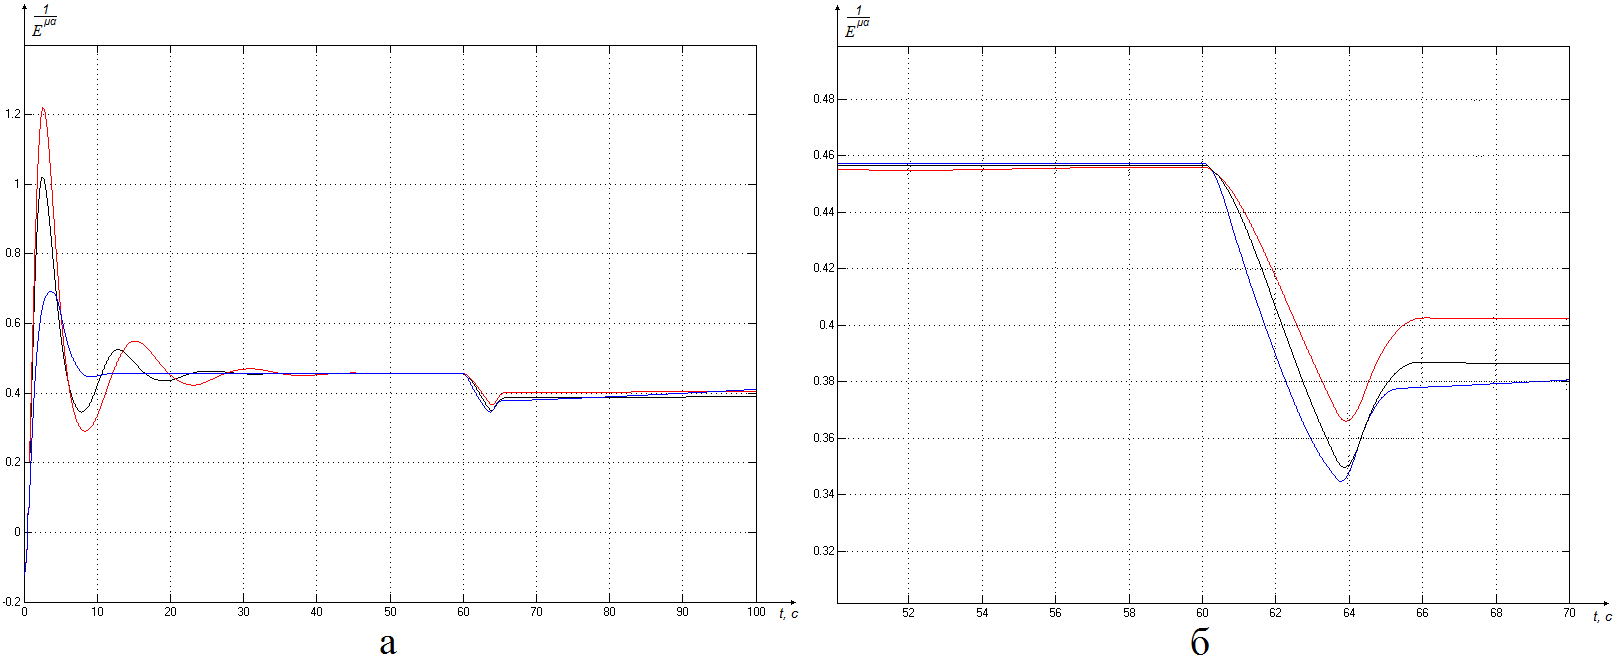
\includegraphics [scale=0.42] {3-6-1.png}
  \caption{Графики изменения величины тягового фактора во время торможения конвейера при различных значениях грузопотока} 
  \label{img:3-6-1}  
\end{figure}

\begin{figure} [h!] 
  \center
  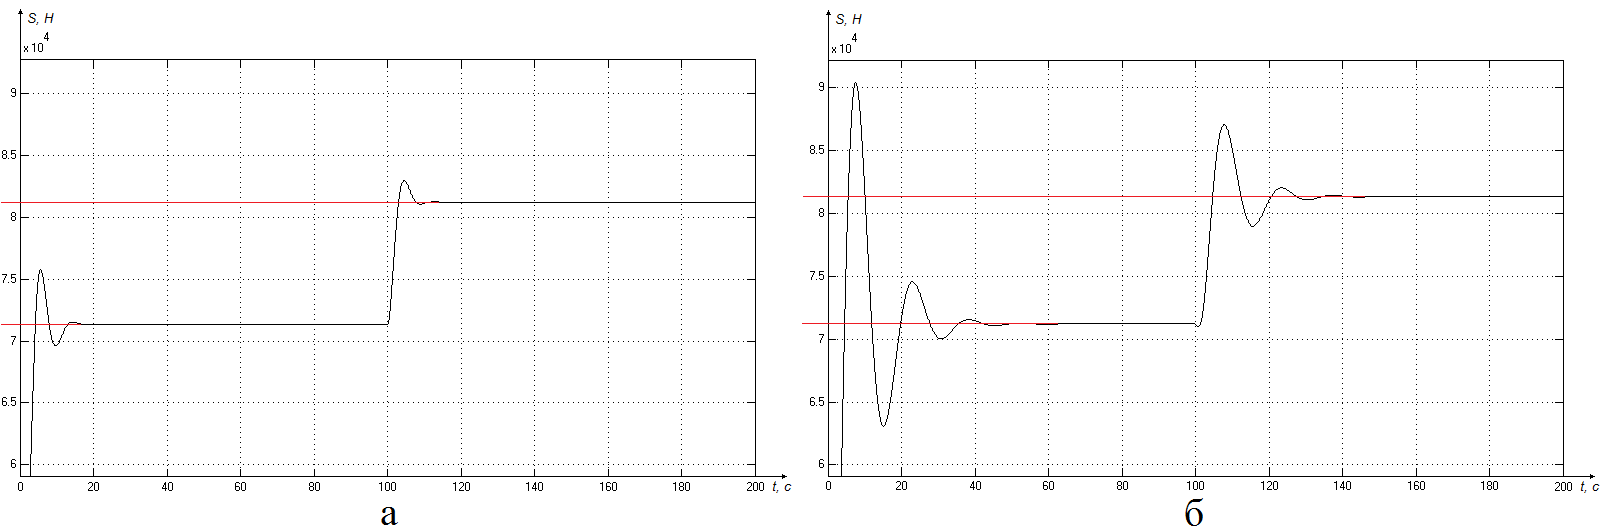
\includegraphics [scale=0.42] {3-6-2.png}
  \caption{Графики изменения величины натяжения ленты в точке набегания на приводной барабан при различных значениях грузопотока} 
  \label{img:3-6-2}  
\end{figure}




\section{Выводы по главе \ref{chapt4}} \label{sect4_7}
В настоящей главе описан общий случай процесса торможения конвейера с использованием колодочных тормозных устройств, и на основе описанных в предыдущей главе исследований разработан алгоритм останова конвейера, основанный на предварительном управляемом торможении хвостового барабана. Применение этого алгоритма позволяет устранить либо минимизировать проскальзывание ленты конвейера на приводном барабане во время его останова. Кроме того, применение этого алгоритма позволяет значительно сократить время останова привода (то есть время, в течение которого проскальзывание ленты в принципе может возникнуть). Например, для исследуемой установки время останова привода при свободном выбеге составляет 4,4 секунды (рис.~\ref{img.3.brake1}), а при останове с использованием разработанного алгоритма время останова привода составляет 0,7 секунды (рис.~\ref{img:4.speeds}). Таким образом, период времени, в течение которого потенциально может возникнуть проскальзывание ленты, сокращается более чем в шесть раз. Кроме того, создаваемые в процессе работы алгоритма останова динамические натяжения в ветвях конвейера фиксируются тормозными устройствами после его останова, что позволяет гарантировано избежать случаев провисания ленты между роликоопорами грузовой ветви. Все это говорит о том, что применение разработанного алгоритма останова конвейера позволяет снизить износ ленты и уменьшить потери транспортируемого груза, а следовательно, повысить эффективность работы конвейерной установки даже в случае неполного устранения проскальзывания ленты.\\

В главе также описана общая методика расчета уставок и параметров, необходимых для работы алгоритма останова конвейера, в зависимости от его характеристик. Методика основывается на найденных в результате модельных исследований зависимостях требуемых параметров от характеристик конвейерной установки и построена таким образом, что может быть применима к любой конвейерной установке в рамках определенного класса.\\

В заключение, в главе описаны исследования изменения натяжений в ленте после останова конвейера посредством отключения тормозных устройств и влияние этого процесса на последующий пуск конвейера. Исследования показывают, что одновременное отключение тормозных устройств при остановленном приводе влечет за собой плавное изменение натяжений в ленте до номинальных значений. Это изменение характеризуется отсутствием колебаний и других нежелательных процессов, которые могли бы повлечь за собой изменение натяжения до такой величины, при которой возможно провисание ленты между роликоопорами грузовой ветви. Это позволяет использовать для последующего пуска конвейера известные алгоритмы, в том числе, и алгоритм со стабилизацией тягового фактора, описанный в работе~\cite{vdmitrieva}.

\if 0
%_______________________________________________________
В разделе~\ref{subsect4_1_2} была определена зависимость, на основе которой возможно рассчитать значение тормозного момента на хвостовом барабане, необходимое для изменения тягового фактора $ \frac{1}{e^{\mu\alpha}} $ до требуемой величины. В разделе~\ref{subsect4_1_2} был проведен расчет и моделирование торможения хвостового барабана конвейера для изменения тягового фактора до величины, равной 0,4, при которой проскальзывание ленты при останове, согласно условию Эйлера, будет отсутствовать.\\

Однако, если смоделировать свободный выбег конвейера~(рис.~\ref{img.3.brake3}), то есть останов с помощью отключения привода без использования торможения, то можно видеть, что величина тягового фактора увеличивается за счет возникающих в ленте динамических усилий, связанных с остановкой движущихся частей конвейера.
В этом случае, в процессе останова привода проскальзывание ленты может иметь место, так как предварительно уменьшенная торможением хвостового барабана величина тягового фактора может превысить значение, определенное условием Эйлера. Для того чтобы этого не происходило, необходимо уменьшать значение тягового фактора с некоторым запасом $ e_\text{доб} $, величину которого требуется определять еще до останова конвейера.

Ниже приведено определение зависимостей установившихся в ленте натяжений после останова привода от значения веса натяжного устройства.

\subsection{Определение зависимостей установившихся в ленте натяжений после останова привода от значения веса натяжного устройства} \label{sect54_2_1}
Определим зависимости установившихся после останова привода натяжений в точках набегания ленты на приводной барабан и сбегания ленты с приводного барабана следующим образом. В модели конвейера меняем вес груза натяжного устройства, производим моделирование останова конвейера посредством свободного выбега и ставим в соответствие текущему весу груза натяжного устройства величины натяжений $ S_1 $ и $ S_4 $, которые установились в ленте после останова привода. Величины натяжений $ S_1 $ и $ S_4 $ будет вычислять на основе их зависимостей от деформаций ленты, полученных в разделе~\ref{sect3_4}. Результаты измерений представлены в табл.~\ref{tabl:5.resultS}.\\

\begin{table}[h!]
\caption{Результаты измерений натяжений ленты после останова привода конвейера при различных значениях веса натяжного устройства.}
\label{tabl:5.resultS}

\begin{center}
\begin{tabular}{|p{0.3\linewidth}|p{0.3\linewidth}|p{0.3\linewidth}|}
\hline
Вес груза натяжного устройства $ G_{\text{ну}}, H $ & Натяжение ленты в точке набегания на приводной барабан $ S_1, H $ & Натяжение ленты в точке сбегания с приводного барабана $ S_4, H $ \\
\hline
20000 & 34750 & 6726  \\
\hline
30000 & 39700 & 11760 \\
\hline
40000 & 44660 & 16770 \\
\hline
50000 & 49620 & 21760 \\
\hline
55000 & 52100 & 24260 \\
\hline
60000 & 54590 & 26750 \\
\hline
65000 & 57080 & 29250 \\
\hline
70000 & 59500 & 31750 \\
\hline
75000 & 62060 & 34240 \\
\hline
80000 & 64560 & 36730 \\
\hline
85000 & 67050 & 39920 \\
\hline
\end{tabular}
\end{center}
\end{table}

На основе данных табл.~\ref{tabl:5.resultS} с использованием метода наименьших квадратов определим зависимость между величиной груза натяжного устройства $ G_\text{ну} $ и натяжением $ S_1 $, возникающем в точке набегания ленты на приводной барабан:

\begin{equation}
\label{eq:4.s1g}
S_1 = f(G_\text{ну}) = 0,5 G_\text{ну} + 24791,51.
\end{equation}

Зависимость между величиной груза натяжного устройства $ G_\text{ну} $ и натяжением $ S_4 $, возникающем в точке сбегания ленты с приводного барабана:

\begin{equation}
\label{eq:4.s2g}
S_4 = g(G_\text{ну}) = 0,5 G_\text{ну} - 3429,87.
\end{equation}


Графики зависимостей представлены на рис.~\ref{img:4.s1s4} (а, б).

\begin{figure}[h!]
  \begin{minipage}[h]{0.49\linewidth}
    \center{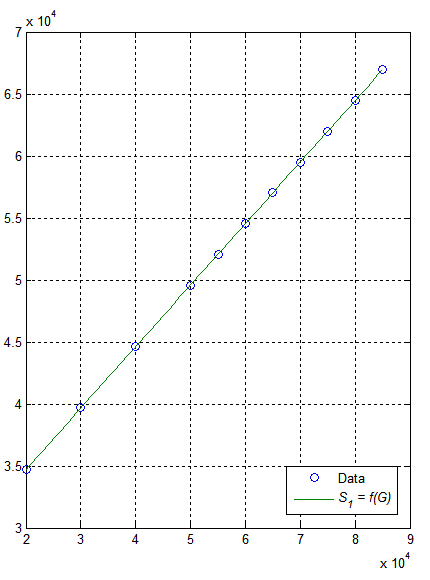
\includegraphics[width=1\linewidth]{4-5.png} \\ а)}
  \end{minipage}
  \hfill
  \begin{minipage}[h]{0.49\linewidth}
    \center{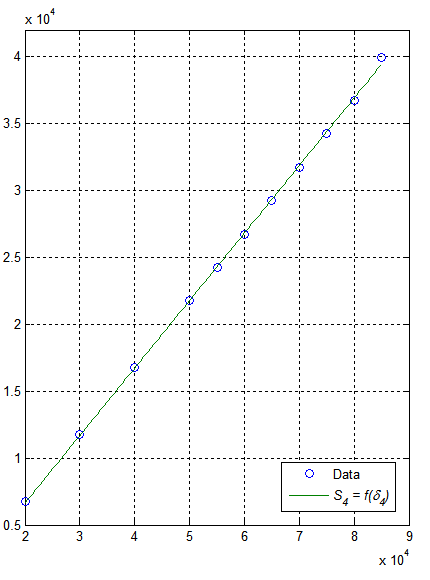
\includegraphics[width=1\linewidth]{4-4.png} \\ б)}
  \end{minipage}
  \caption{Графики зависимости натяжений ленты после останова привода конвейера от веса груза натяжного устройства}
  \label{img:4.s1s4}  
\end{figure}

На основе определенных зависимостей могут быть вычислены натяжения в ленте после останова привода, а следовательно, и установившаяся величина тягового фактора  $ \frac{1}{e^{\mu\alpha}_\text{уст}} $. Тогда величину запаса $ e_\text{доб} $ можно определить следующим образом:

\begin{equation}
\label{eq:4.edob}
e_\text{доб} = \frac{1}{e^{\mu\alpha}_{\text{уст}}} - \frac{1}{e^{\mu\alpha}_{\text{ном}}}
\end{equation}

\subsection{Расчет требуемого значения тягового фактора и тормозного момента для обеспечения останова конвейера без проскальзывания ленты} \label{sect54_2_2}
%_______________________________________________________
\fi
